\chapter*{Prólogo}
\addcontentsline{toc}{chapter}{Prólogo}

Durante mucho tiempo nos preguntamos cómo diseñar un curso de Algoritmos y Programación I
(primera materia de programación de las carreras de Ingeniería en Informática y Licenciatura
en Análisis de Sistemas de la Facultad de Ingeniería de la UBA) que al mismo tiempo fuera
atractivo para los futuros profesionales de la informática, les permitiera aprender a resolver
problemas, y atacara muy directamente el problema de la deserción temprana de estudiantes.


Muchos de los estudiantes que ingresan a primer año de las carreras de informática en nuestro
país lo hacen sin saber programar pese a ser nativos digitales, para los cuales las computadoras
y muchos programas forman parte de su vida cotidiana. El primer curso de programación plantea
entonces varios desafíos: enseñar una metodología para la resolución de problemas, un lenguaje
formal para escribir los programas, y al mismo tiempo hacer que los estudiantes no se sientan
abrumados, tengan éxito en este primer esfuerzo y se sientan atraídos por la posibilidad de
escribir sus propios programas.


En este sentido, la elección del lenguaje de programación para dicho curso no es un tema menor:
el problema radica en elegir un lenguaje que al mismo tiempo sea suficientemente expresivo, tenga
una semántica clara y cuyas complicaciones sintácticas sean mínimas.


Hacía tiempo que buscábamos un lenguaje con todas estas características cuando, durante el debate
posterior a un panel sobre programación en el nivel que tuvo lugar en la conferencia Frontiers in
Engineering Education 2007 organizada por la IEEE, el Dr. John Impagliazzo, de Hofstra University,
relató cómo sus cursos habían pasado de duras experiencias, con altas tasas de deserción, a una
situación muy exitosa, por el solo hecho de haber cambiado el lenguaje de programación de ese curso
de Java a Python. Después de ese estimulante encuentro con Impagliazzo nos pusimos manos a la obra
para diseñar este curso. Fue una grata sorpresa enterarnos también de que el venerable curso de
programación de MIT también había migrado a Python: todo hacía pensar que nuestra elección de lenguaje
no era tan descabellada como se podía pensar.


Este libro pretende entonces ser una muy modesta contribución a la discusión sobre cómo enseñar a
programar en primer año de una carrera de Informática a través de un lenguaje que tenga una suave
curva de aprendizaje, de modo tal que este primer encuentro le resulte a los estudiantes placentero
y exitoso, sin que los detalles del lenguaje los distraiga del verdadero objetivo del curso: la resolución
de problemas mediante computadoras.


Queremos agradecer a la Facultad de Ingeniería (en particular a su Comisión de Publicaciones)
por la publicación de este libro. Y también a todos los que apoyaron desde un primer momento
la escritura y mejora continua de lo que fueron durante varios años las notas de nuestro curso de
Algoritmos y Programación I: a la Comisión Curricular de la Licenciatura en Análisis de Sistemas y al
Departamento de Computación (y a su director, Gustavo López) por apoyar la iniciativa de dar este curso
como piloto, a quienes leyeron y discutieron los manuscritos desde sus primeras versiones y colaboraron
con el curso (Melisa Halsband, Alberto Bertogli, Sebastián Santisi, Pablo Antonio, Pablo Najt, Diego Essaya,
Leandro Ferrigno, Martín Albarracín, Gastón Kleiman, Matías Gavinowich), a quienes fueron primero alumnos y
luego colaboradores de esta experiencia educativa (Bruno Merlo Schurmann, Damian Schenkelman, Débora Martín,
Ezequiel Genender, Fabricio Pontes Harsich, Fabrizio Graffe, Federico Barrios, Federico López, Gaston
Martinez, Gaston Goncalves, Ignacio Garay, Javier Choque, Jennifer Woites, Manuel Soldini, Martín Buchwald,
Pablo Musumeci), a los amigos que, como Pablo Jacovkis, Elena García y Alejandro Tiraboschi se ofrecieron a
revisar manuscritos y a hacer sugerencias, y a todos los alumnos de nuestro curso de Algoritmos y
Programación I de la FIUBA que, desde 2009, han usado este texto y nos han ayudado a mejorarlo permanentemente.
De todos modos, por supuesto, los errores son nuestra responsabilidad.

\vspace{1cm}
\hfill Buenos Aires, diciembre de 2012.

\section*{Segunda edición}

Habiendo dictado el curso de Algoritmos y Programación I durante
varios años ya, podemos felizmente decir que el curso ya no es más \enquote{piloto},
y conseguimos en el camino una buena cantidad de logros.

Al final de cada cuatrimestre presentamos a los alumnos una encuesta de
satisfacción, en la que tanto el curso como el apunte recibieron
mayoritariamente buenas
críticas\footnote{Los resultados de las encuestas están publicados en
\url{https://algoritmos1rw.ddns.net/encuestas}}. A continuación se muestra el
resultado de dos de las preguntas incluidas en las encuestas.

\begin{center}
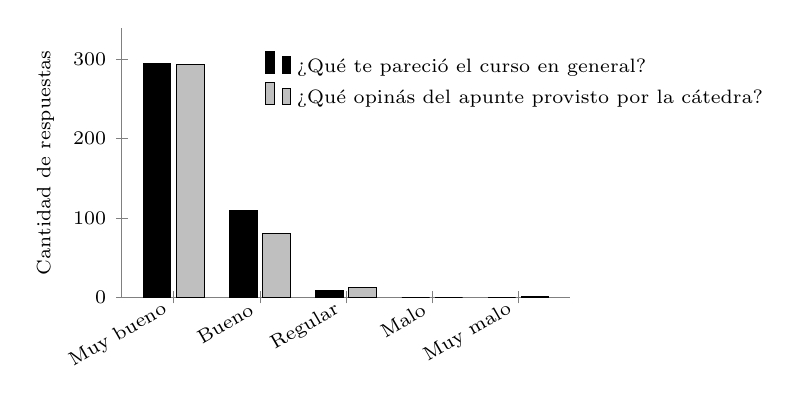
\begin{tikzpicture}
\begin{axis}[
ybar,
axis x line={bottom},
axis y line={left},
axis line style={-,gray},
enlarge x limits=0.15,
enlarge y limits={0.15,upper},
legend style={draw=none,at={(0.3,0.8)},font=\scriptsize,anchor={west}},
legend cell align={left},
ylabel={Cantidad de respuestas},
ylabel style={font=\scriptsize},
symbolic x coords={Muy bueno,Bueno,Regular,Malo,Muy malo},
xtick=data,
x tick label style={rotate=30,anchor=east,font=\scriptsize},
y tick label style={font=\scriptsize},
width=0.6\textwidth,
height=5cm,
]
\addplot[black,fill=black] coordinates {(Muy bueno,295) (Bueno,110) (Regular,8) (Malo,0) (Muy malo,0)};
\addplot[black,fill=black!25] coordinates {(Muy bueno,293) (Bueno,81) (Regular,12) (Malo,0) (Muy malo,1)};
\legend{¿Qué te pareció el curso en general?,¿Qué opinás del apunte provisto por la cátedra?}
\end{axis}
\end{tikzpicture}
\end{center}

Debido a la buena aceptación que tuvo el curso, en 2014 se dio el reconocimiento
de que la Comisión Curricular de la Licenciatura en Sistemas adoptara el temario
desarrollado por el curso como programa del plan de estudios oficial,
actualización que aprobó el Consejo Superior ese mismo año.  También en 2014
se comenzaron a dictar cursos de Introducción a la Programación en Python que
utilizan la planificación del curso, aprobados por el Consejo Directivo.

En paralelo con todo esto fuimos mejorando el apunte: arreglando erratas,
mejorando redacciones, y agregando y actualizando temas. El cambio más
importante fue la actualización a la versión 3 de Python, que decidimos hacer
entre otras razones porque Python 2 será discontinuado en 2020. Entre los
temas adicionados figuran: diseño de funciones recursivas, composición y mutabilidad
de objetos, funciones de orden superior, listas por comprensión, la instrucción
|import|, conjuntos. Además se mejoró la redacción general de todos los capítulos,
y se reorganizó la guía de ejercicios. Todas estas mejoras se incluyen en esta
Segunda Edición.

Por último, extendemos la lista de agradecimientos a todos aquellos que
fueron alumnos y luego colaboradores del curso a lo largo de los últimos años:
Agustín Santiago,
Agustina Mendez,
Alan Rinaldi,
Alejandro Levinas,
Ana Czarnitzki,
Ariel Vergara,
Ayelén Bibiloni Lombardi,
Carlos Talavara,
Constanza Gonzalez,
Daniela Riesgo,
Daniela Soto,
Diego Alfonso,
Emiliano Sorbello,
Eugenia Mariotti,
Federico Esteban,
Florencia Álvarez Etcheverry,
Florencia Rodriguez,
Franco Di María,
Gianmarco Cafferatta,
Ignacio Sueiro,
Joel Saidman,
Juan Costamagna,
Juan Ignacio Kristal,
Juan Patricio Marshall,
Julián Crespo,
Klaus Lungwitz,
Lucas Perea,
Luciano Sportelli Castro,
Manuel Battan,
Manuel Porto,
Manuel Sturla,
Martín Coll,
Martín Dabat,
Matías Scacosky,
Maximiliano Suppes,
Maximiliano Yung,
Miguel Alfaro,
Milena Farotto,
Nicolás Poncet,
Ramiro Santos,
Robinson Fang,
Rodrigo Velez,
Sebastián Gonzalez,
Sofía Morseletto,
Tomás Rocchi.

\vspace{1cm}
\hfill Buenos Aires, agosto de 2018
